%The arial font needs either XeTex or LuaTex to work. Change the typesetting engine to xelatex or lualatex
%if an error is displayed when running the code.

\documentclass[10pt]{standalone}
\usepackage{tikz}
\usepackage{verbatim}
%\renewcommand{\familydefault}{\sfdefault}
\usepackage{fontspec}
\setmainfont{Arial}

\usetikzlibrary{arrows,positioning} 
\tikzset{
%Define standard arrow tip
    >=stealth',
%Define style for boxes
    punkt/.style={
           rectangle,
           rounded corners,
           draw=black, thick,
           text width=8em,
           minimum height=2em,
           text centered},
     punkt2/.style={
           rectangle,
           rounded corners,
%draw=black, thick,
           text width=18em,
           minimum height=2em,
           text centered},
    circle2/.style={
           circle,
           rounded corners,
           draw=black, thick,
           text width=5em,
           minimum height=2em,
           text centered},
% Define arrow style
    pil/.style={
           ->,
           thick,
           shorten <=2pt,
           shorten >=2pt,},
    pol/.style={
           <-,
           thick,
           shorten <=2pt,
           shorten >=2pt,}
}

\begin{document}

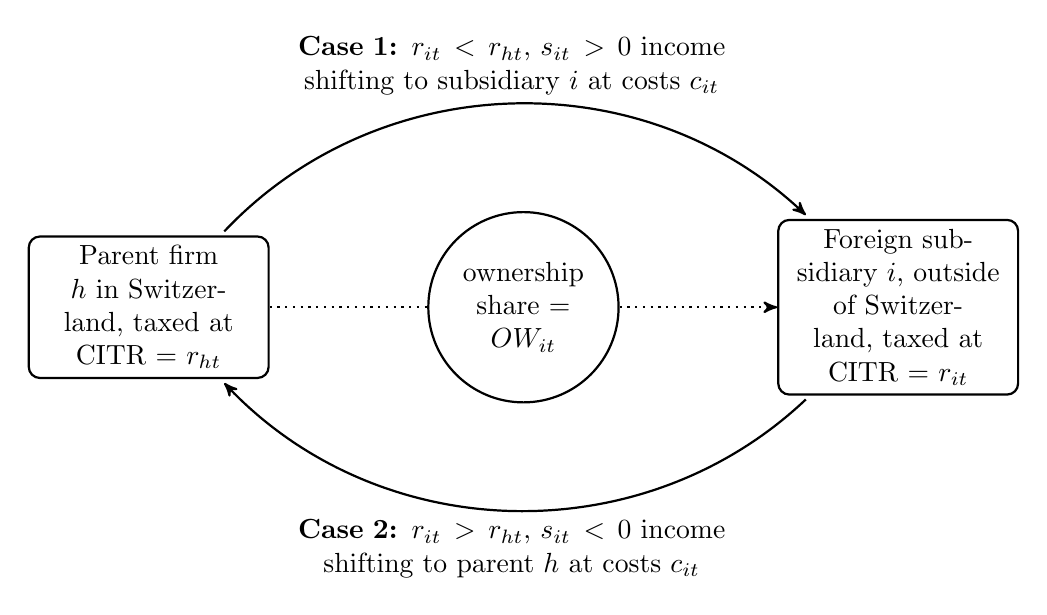
\begin{tikzpicture}[node distance=2cm, auto,]
 (formidler) {Intermediaries (c) balsdf sdf as asdf asdf asfd asdf };
 \node [circle2] (dummy) {ownership share = $OW_{it}$};
 \node[right=of dummy] [punkt] (F) {Foreign subsidiary $i$, outside of Switzerland, taxed at CITR = $r_{it}$};
 \node[left=of dummy] [punkt] (g) {Parent firm $h$ in Switzerland, taxed at CITR = $r_{ht}$}
   edge[pol, bend right=45] node[below] [punkt2]{\textbf{Case 2:} $r_{it}>r_{ht}$, $s_{it}<0$ income shifting to parent $h$ at costs $c_{it}$} (F)
   edge[pil, bend left=45] node[above] [punkt2]{\textbf{Case 1:} $r_{it}<r_{ht}$, $s_{it}>0$ income shifting to subsidiary $i$ at costs $c_{it}$} (F);
   \draw[dotted] [->, thick] (dummy) -- (F);
   \draw[dotted] [-, thick] (g) -- (dummy);
\end{tikzpicture}

\end{document}

